\documentclass[]{scrartcl}

\usepackage{graphicx}
\usepackage{float}

%opening
\title{Multi-Agent Systems Assignment 6}
\author{Alex Hoorn, student 2716056}

\begin{document}

\maketitle

\section{Monte Carlo Sampling}

In this task we consider choosing a house to rent as a sequential decision problem. We visit $n$ houses. After every visit we must make the choice to either rent the house or leave it. We cannot come back to a previously visited place.

To get a distribution of house rating we use Monte Carlo sampling. Here $X$ is sampled from a standard normal distribution. Then we run every $x \in X$ through a function $f(x)$ to get the actual distribution of the house ratings. I have defined $f(x)=\sin^2(x)$.

\begin{figure}[H]
	\centering
	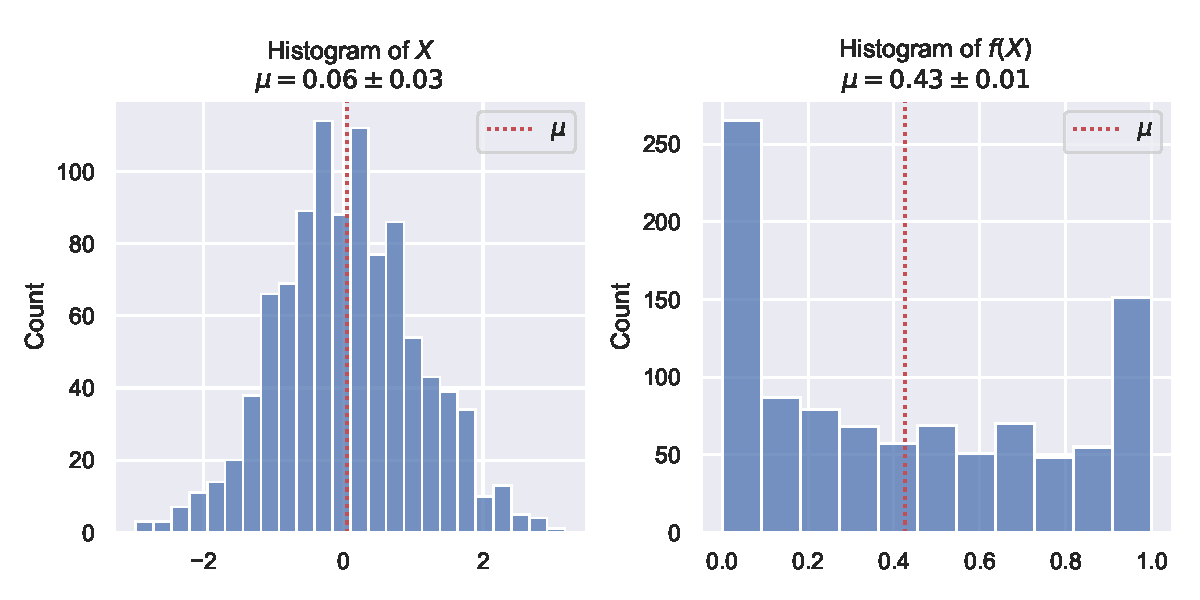
\includegraphics[width=0.7\linewidth]{1-1.pdf}
	\caption{Monte Carlo sampling.}
	\label{fig:1-1}
\end{figure}

The strategy I used to pick a house is based on the Law of Large Numbers\footnote{https://en.wikipedia.org/wiki/Law\_of\_large\_numbers}---LLN in short.
I determine an expected utility after $n$ observations. And then simply pick the first observation which is better than the expectation.

\begin{figure}[H]
	\centering
	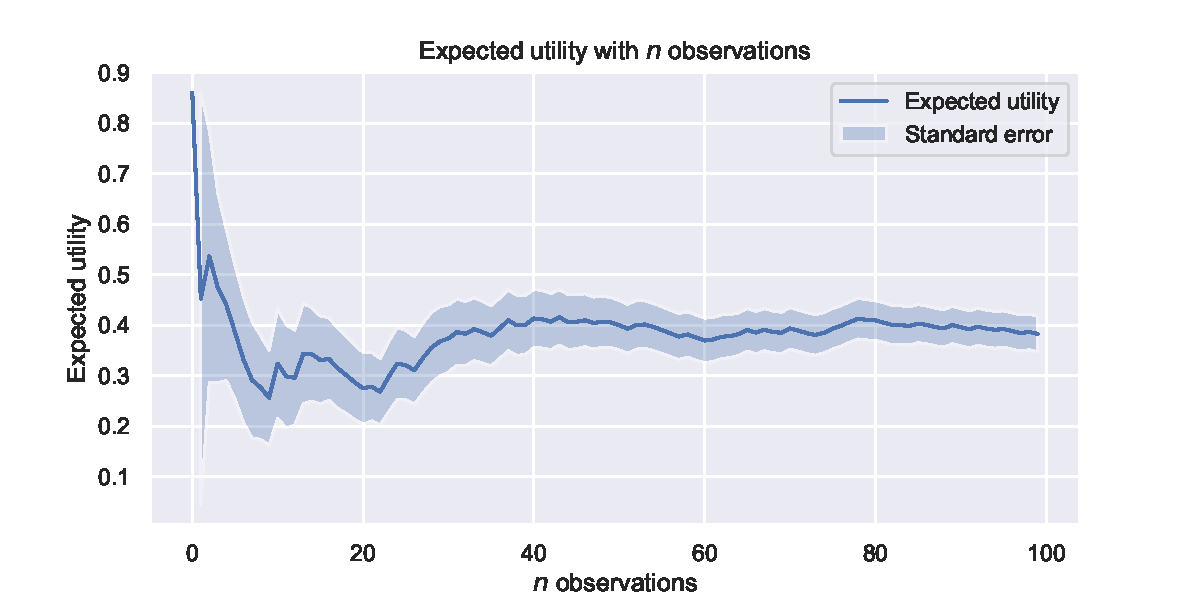
\includegraphics[width=0.7\linewidth]{1-2.pdf}
	\caption{The Law of Large Number visualized for $f(X)$.}
	\label{fig:1-2}
\end{figure}

If simply taking the mean of the results into account then this strategy performs very well. Starting from a mean of about 0.75. However, I have noticed that the results of this strategy varies wildly in practice and thus probably shouldn't actually be relied on. In Figure \ref{fig:1-3} we can see that the range of the expected rewards is always rather large for any $n$, i.e. for $n=200$ the range is $[0.4, 1.0]$.

\begin{figure}[H]
	\centering
	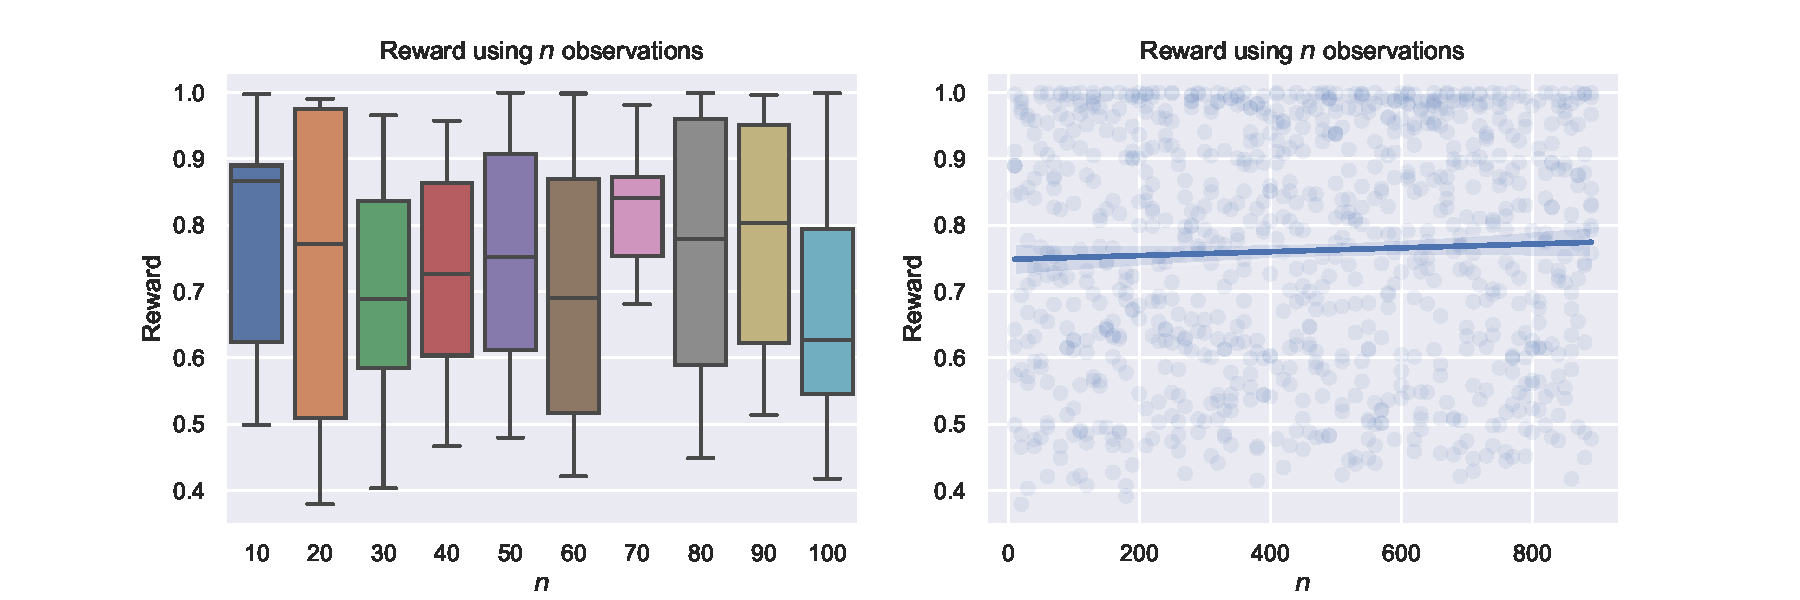
\includegraphics[width=1\linewidth]{1-3.pdf}
	\caption{Results using the strategy ``pick first $> e$''.}
	\label{fig:1-3}
\end{figure}

\section{Monte Carlo Tree Search}

To develop and try out my Tree Search algorithm I have implemented a very basic class to supply the logic behind the binary tree. This class doesn't actually generate a whole tree on creation. Instead, it generates a target path and lazily calculates a reward only when asked. The benefit of this approach is that the tree can be (pretty much) of infinite size. However, in my testing I still limited it to a tree with a depth of 25.

The rewards are calculated using $x_i = Be^{-d_i/r}$. $d$ is the edit distance between the path and the target set in the tree. $B$ and $r$ have been set to 2 and 20 respectively to make differences between different paths of nodes that are alike non-negligible.

One big difference between the default MCTS implementation and mine is that when a new node is reached its direct children are immediately rolled out. Instead of waiting for a new iteration that would select the child node (very often) anyway. This is much easier to do programmatically instead of dealing with unexplored children and divisions by zero.

Doing this adds some performance impact. To regain this I have implemented an early-stopping method. This makes it so that for selecting every new root node the algorithm doesn't have to iterate to its full allotted budget (e.g. 50 iterations). If it hits leaf nodes a set amount of times the iterations are cut short and a new root node is returned.

MCTS traverses a tree by calculating the UCB-value of nodes. This is calculated by $U C B(\textrm{node}_{i})=\bar{x}_{i}+c \sqrt{\frac{\log N}{n_{i}}}$. I have noticed that the tunable parameter $c$ in this  formula plays a huge role in finding the optimal reward in a tree. With a high $c$ the algorithm is more likely to reach unexplored areas of the tree. This makes it more likely to find the optimal solution at the cost of additional iterations necessary to do so (and therefore runtime). The results are shown in Figure \ref{fig:2-1}.

\begin{figure}[H]
	\centering
	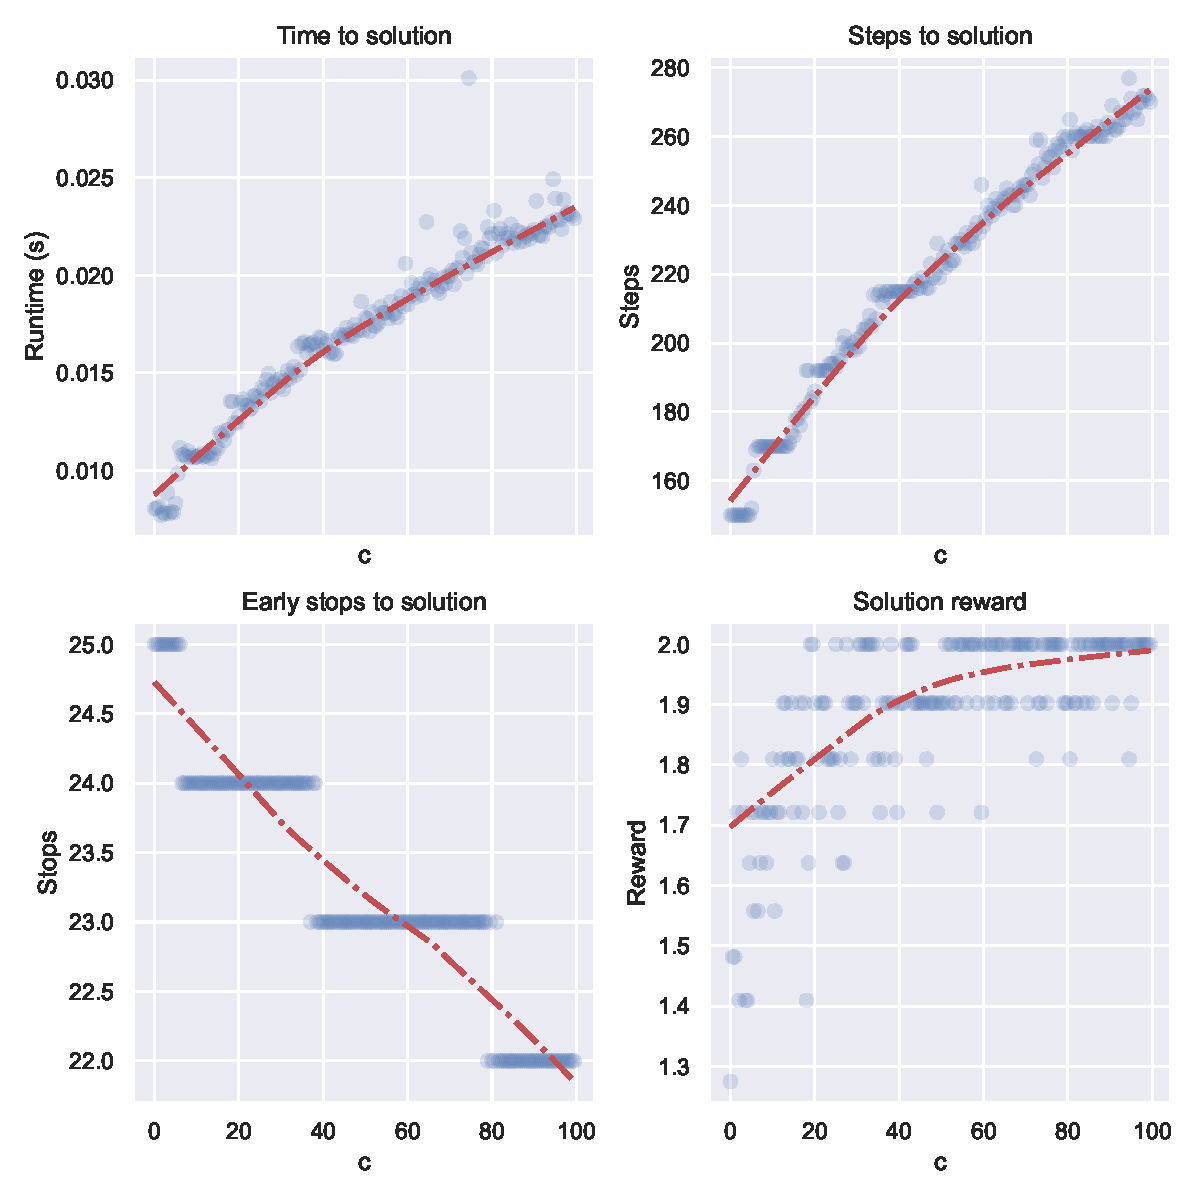
\includegraphics[width=0.7\linewidth]{2-1.pdf}
	\caption{Statistics for different settings of $c$ with 5 roll-outs and 50 iterations.}
	\label{fig:2-1}
\end{figure}


\section{Reinforcement Learning}

In this task we consider a $9\times9$ grid world as depicted in Figure \ref{fig:3-0}. The blue cells denote inaccessible walls. The green cell is a terminal cell which rewards 50 and the red cell is a terminal cell that yields -50. Any transition to a different state costs -1. The grid world is evaluated with three different reinforcement learning algorithms:

\begin{itemize}
	\item Monte Carlo Sweep \textit{with equiprobable policy.}
	\item Greedy SARSA.
	\item Q-Learning.
\end{itemize}

\begin{figure}[H]
	\centering
	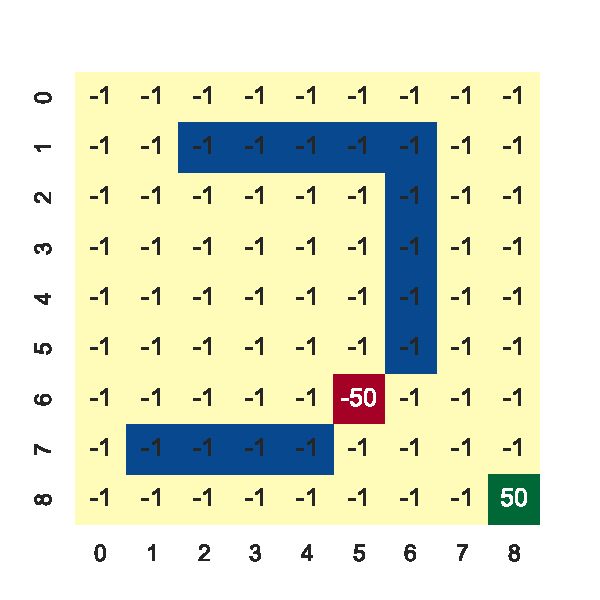
\includegraphics[width=0.4\linewidth]{3-0.pdf}
	\caption{The environment, blue denotes walls, red and green are terminal states.}
	\label{fig:3-0}
\end{figure}

\subsection{Monte Carlo Sweep}

The Monte Carlo evaluation in combination with the equiprobable policy means that the agent simply \textit{wanders around} the grid world until it reaches a terminal state. There is no clever selection of the action to take. The agent could even attempt to walk off the grid or against walls. This results in very low returned rewards, because for every transition the total reward is lowered by -1. The results for this evaluation is shown in Figure \ref{fig:3-1}.

\begin{figure}[H]
	\centering
	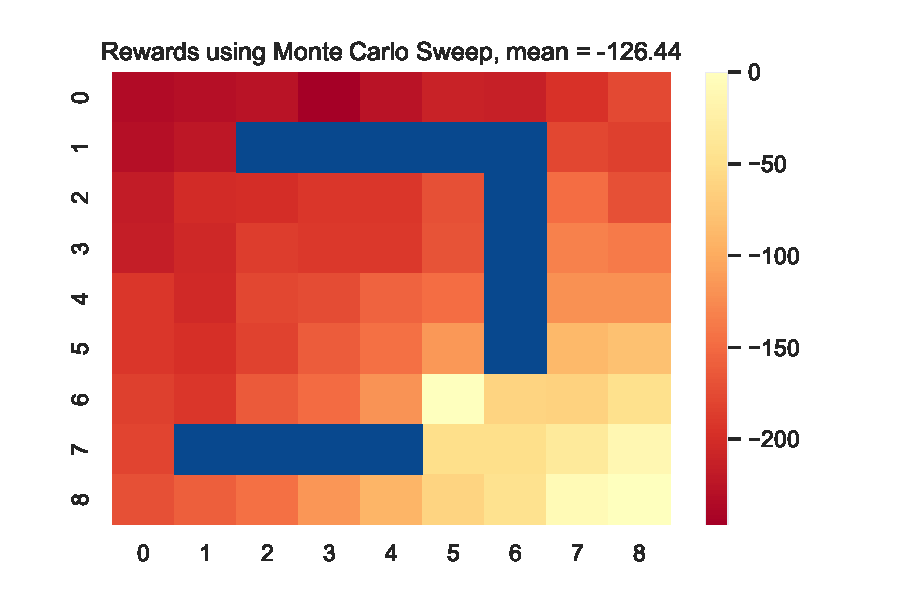
\includegraphics[width=0.5\linewidth]{3-1.pdf}
	\caption{Heatmap of Monte Carlo Sweep.}
	\label{fig:3-1}
\end{figure}

\subsection{Greedy SARSA and Q-Learning}

Compared to the Monte Carlo Sweep the SARSA and Q-Learning algorithms are much smarter. These will not wander around aimlessly but actively follow a path to the best reward. With a chance defined by parameter $\epsilon$ will a random action be taken rather than an optimal action ($\epsilon$-greedy).

The only difference between SARSA and Q-Learning is how they update their values along the way. For SARSA the values are updated with:
$$Q(s, a) \leftarrow Q(s, a)+\alpha\left[r+\gamma Q\left(s^{\prime}, a^{\prime}\right)-Q(s, a)\right]$$

For Q-Learning we use:
$$Q(s, a) \leftarrow Q(s, a)+\alpha\left[r+\gamma \max_a Q\left(s^{\prime}, a\right)-Q(s, a)\right]$$

In the actual implementation Q-Learning completely inherits the SARSA class. It only changes the update method.

Because SARSA picks $a^\prime$ using the $\epsilon$-greedy policy it is called on-policy. Q-Learning greedily updates with $\max_a$, therefore it is called off-policy as it does not follow the $\epsilon$-greedy policy.

The results after 1000 episodes with $\epsilon = 0.1$, $\alpha = 0.2$ and $\gamma = 0.9$. Are shown in Figure \ref{fig:3-2}. It can be seen that the results are very much the same except for some pathing specifics. This can easily be explained by the fact that SARSA and Q-Learning are very much the same algorithms, except for one specific detail in the updating rule.

In some runs it could be seen that the path from one cell above the +50 reward with either SARSA or Q-Learning was not directly to the reward. Instead, it unexpectedly went around it. However, this was not often observed so this is most likely a pure coincidence because of $\epsilon=0.1$. But still interesting that it can happen.

\begin{figure}[H]
	\centering
	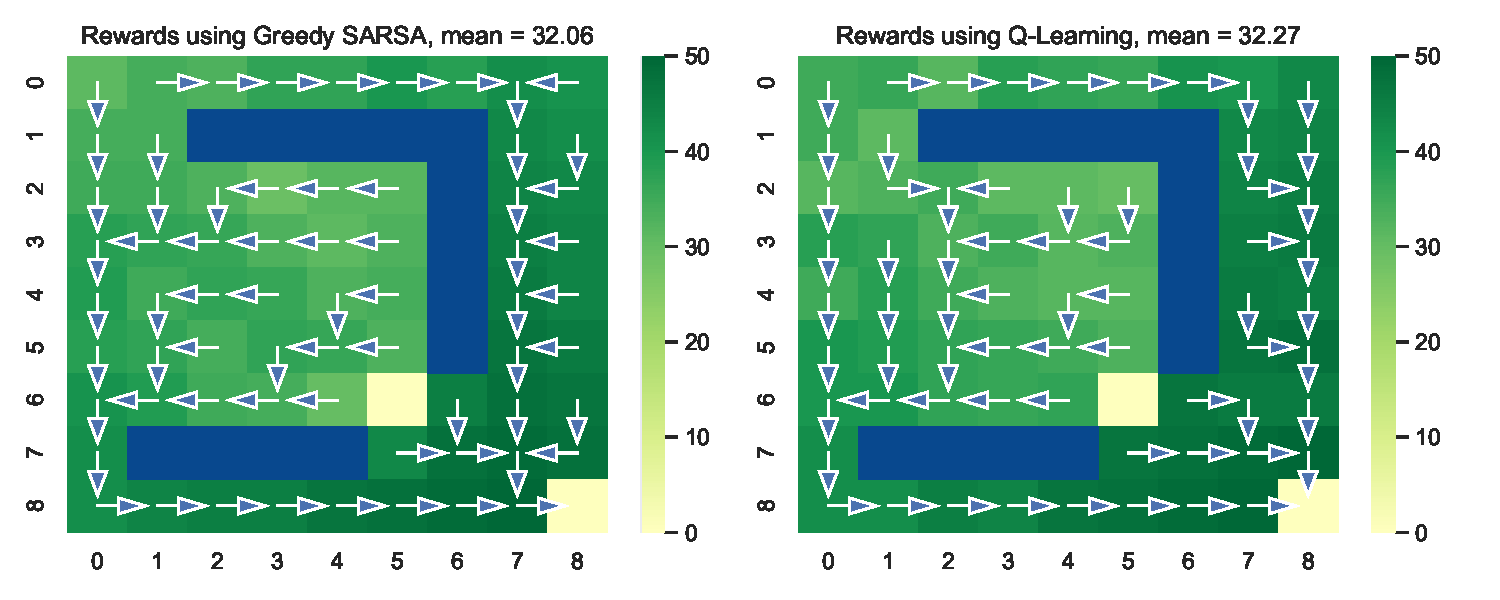
\includegraphics[width=0.8\linewidth]{3-2.pdf}
	\caption{Heatmaps with path of Greedy SARSA (left) and Q-Learning (right)}
	\label{fig:3-2}
\end{figure}

To try to understand a bit more about the different inner workings of SARSA and Q-Learning I compared their performances over an array of episodes. I was expecting Q-Learning to converge slightly faster on some optimal reward due to it updating with $\max_a$. But this does not seem the case as seen in the right plot of Figure \ref{fig:3-3}. Perhaps the grid world example is not complex enough to show a difference between the two methods.

\begin{figure}[H]
	\centering
	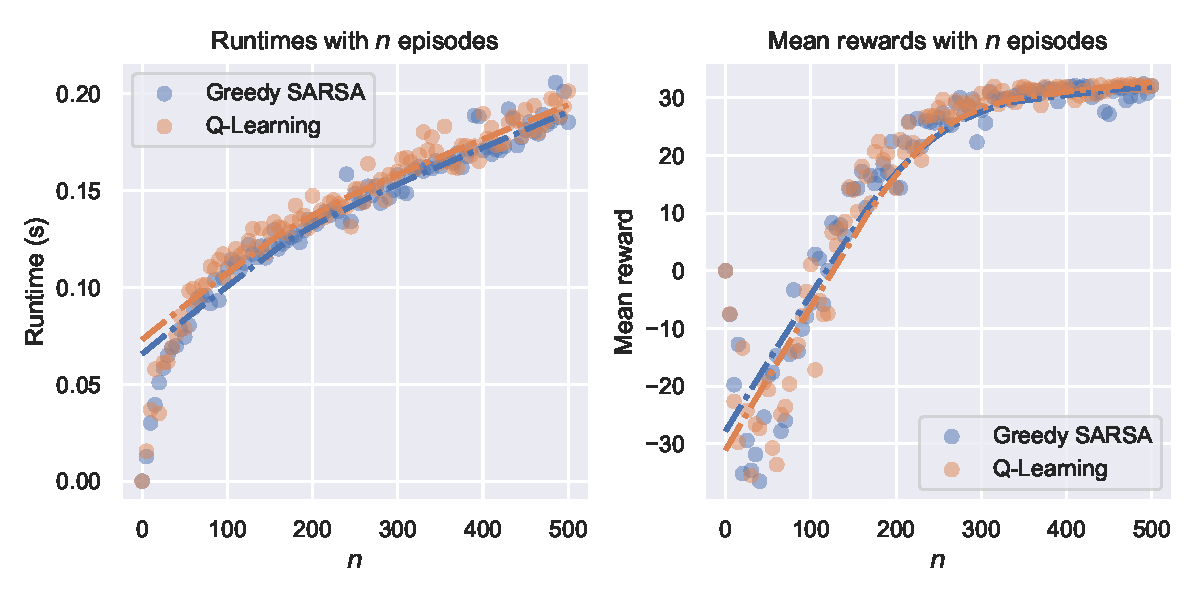
\includegraphics[width=0.7\linewidth]{3-3.pdf}
	\caption{Performance of SARSA and Q-Learning with $n$ episodes.}
	\label{fig:3-3}
\end{figure}

\end{document}
